In this chapter, we extend the metadynamics simulation to a binary Lennard-Jones liquid.  The Kob-Andersen model is a known glass former.  By applying metadynamics to both a fragile glass former (Kob Andersen model) and a poor glass former (monoatomic Lennard-Jones), we can get a more thorough understanding of the energy landscape.  Herein, we define a good glass former (the fragile glass forming system) as a system that is likely to form a glassy state without extreme conditions applied to frustrate the crystal state.  We define a poor glass former, or a good crystal former (the monoatomic Lennard-Jones system), as a system that is likely to equilibrate to the crystal state, and therefore not likely to form a glassy system unless extreme conditions are applied to frustrate the crystal state.  These definitions are to help the reader.

\section{Theory and Background}
As discussed in Chapter \ref{metadynamics}, the energy landscape has been a highly successful picture for detailing the behavior of materials both in and out of equilibrium, the relaxation of metastable materials, and the difference between alpha and beta relaxations \cite{Royall2015}.  However, as a theoretical concept, the energy landscape is difficult to prove with any experimental evidence.  There is no physical or experimental method that can directly sample the energy landscape.  Further, due to the high dimensionality of the energy landscape, detailing the full energy landscape is difficult from simulations as well.  Thus, despite a large amount of recent work using the energy landscape to explain physical phenomena, no direct evidence exists to proof what we believe the landscape to look like.  

As previously discussed, it is believed that the energy basin for the crystal state is narrow and extremely deep (generally the deepest basin on the landscape, depending on the number of crystal polymorphs \cite{De2014}).  Similarly, it is often theorized that metastable basins are deep while not as deep as the crystal state, and often described as broad \cite{De2014}.  The glassy basins are described as rich with small and large energy minimums separating the multitude of energy minimums within a local region of the landscape \cite{De2014}.  However, since the landscape has generally remained a theoretical framework, the distinction between landscapes of glass formers and crystal formers has remained merely theoretical.  

We have already shown the potential of metadynamics to sample a trajectory along the energy landscape.  Thus, by employing the metadynamics method we have implemented, we can directly sample the energy landscape of a good glass former and a good crystal former and determine the actual difference between the two landscapes.  We have already shown the density effects on the landscape.  Now, we show unique features between a good crystal and good glass former.

\section{Results}
\label{kob_andersen}
Metadynamics was applied to two distinctly different systems, a monoatomic Lennard-Jones argon and a binary Lennard-Jones system.  The monoatomic Lennard-Jones system is identical to the system used in the previous chapter for studying nucleation and crystal growth.  The system was composed of 864 Lennard-Jones argon atoms, with parameters $\sigma = .340$, and $\epsilon = .9977$.  The metadynamics parameters used were penalty height of 1 kJ/mol, a height squared of .1 nm$^2$, a maximum number of penalties of 20,000, a initial minimization step of .0001 nm, and the structural restraints were disabled.  The binary Lennard-Jones system was composed of 178 atoms of type A and 45 atoms of type B, or roughly a ratio of 80:20, the Lennard-Jones parameters were $\sigma_{AA} = .340$, $\sigma_{BB} = .299$, $\sigma_{AB} = .272$, $\epsilon_{AA} = .9977$, $\epsilon_{BB} = .4989$, $\sigma_{AB} = 1.4966$ \cite{PhysRevE.51.4626}.  This is the well known Kob-Andersen system \cite{PhysRevE.51.4626}, and is a well known glass forming system.  The metadynamics simulation parameters were a penalty height of 1 kJ/mol, penalty width squared of .1 nm$^2$, a maximum number of penalties of 2,000,000, an initial minimization step of.001.  The monoatomic system was simulated for 2 hours with 12 processors, and the binary Lennard-Jones system was simulated for 20 hours with 12 processors.  The difference is because the nucleation and crystallization process completes quickly on the monoatomic system.  The potential energy sampled by the two simulations are shown in Figure \ref{compare_landscape}.

\begin{figure}[h]
	\centering
	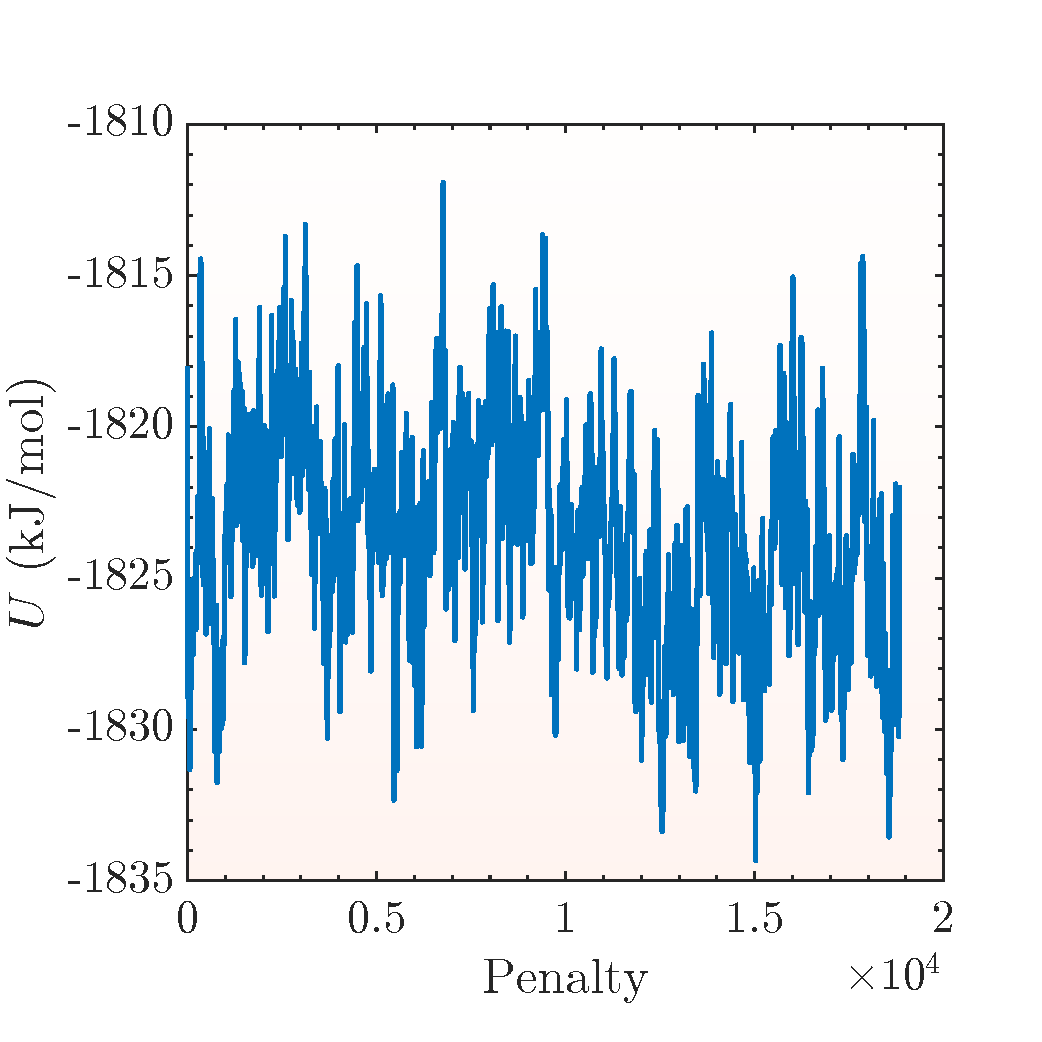
\includegraphics[width=.45\textwidth]{./Figures/Landscape/glassy_landscape.pdf}
	\hspace{.01\textwidth}
	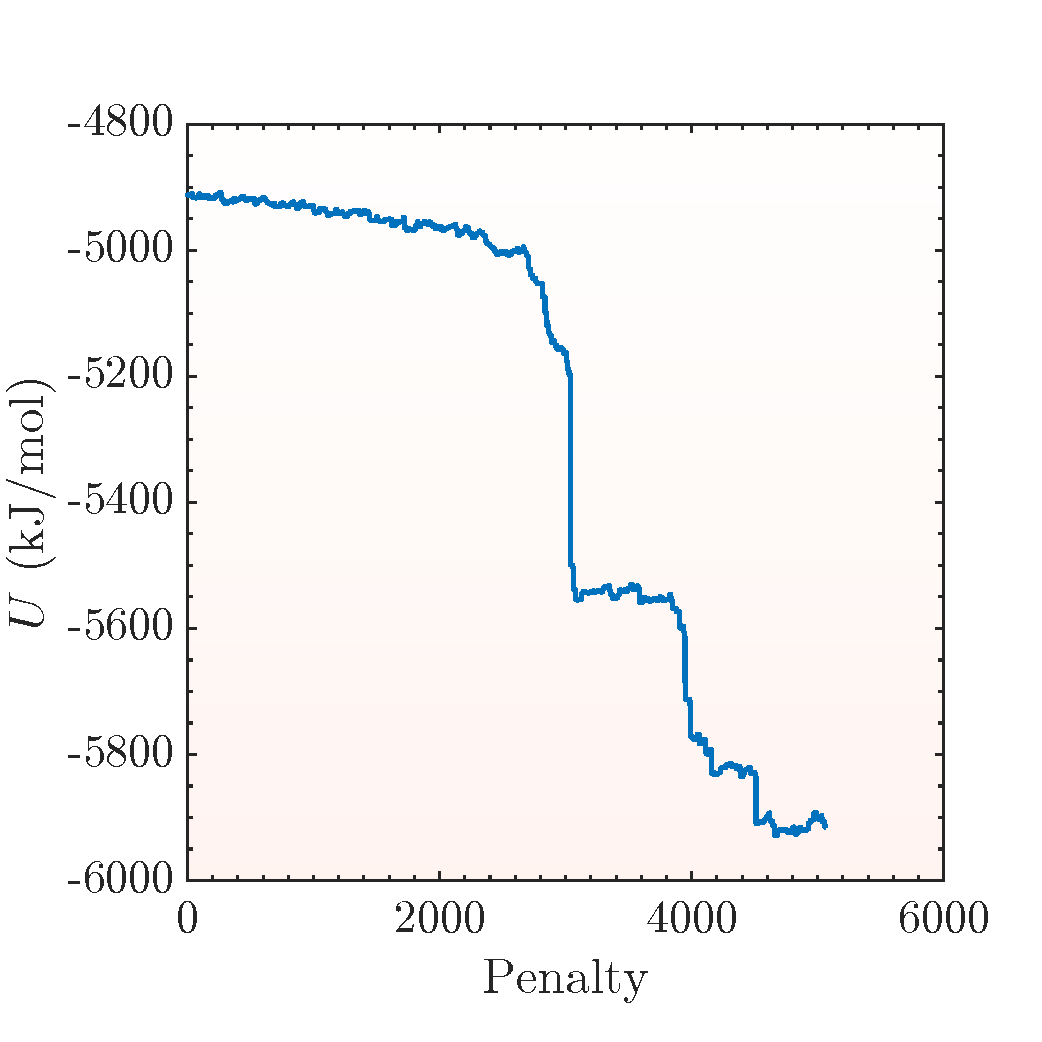
\includegraphics[width=.45\textwidth]{./Figures/Landscape/crystal_landscape.pdf}
	\caption{Potential Energy versus penalty number for two simulations.  The left figure shows the potential energy sampled for a binary Lennard-Jones system known for being a fragile glass former.  The right figure shows the potential energy landscape sampled for a monoatomic Lennard-Jones system known for being a poor glass former.}
	\label{compare_landscape}
\end{figure}

Figure \ref{compare_landscape} shows the energy landscapes sampled by the two simulations.  The left figure shows the binary Lennard-Jones system and the right one shows the monoatomic Lennard-Jones.  The first major aspect to notice is the difference in scales.  The monoatomic system has only 5000 penalties applied whereas the binary system has nearly 20,000 penalties applied.  This is due to the fact that the monoatomic system had a finite duration, added more penalties once it was in the deep crystal minimum only resulted in vibrations of the crystal lattice, thus applying more penalties resulted in extraneous information.  This helps prove that the crystal state minimum is deep and narrow, because even after adding many more penalties the system never began to re-climb out of the minimum, we never saw the system become disordered again.  Conversely, the binary system required the application of as many penalties as possible in order to get thorough sampling of the entire landscape.  We needed good statistics of the landscape for a separate analysis of this system.  When viewing the real space movie of the binary system and when looking at the bond order parameter, the system never showed signs of order.  

The next major observation to make about the two landscapes is that for the monoatomic system, the potential energy generally only decrease after overcoming a barrier.  This is indicative of a funnel like landscape.  The landscape is rather simple and the gradient of the landscape ubiquitously points downwards towards the crystal state.  Comparatively, the binary system landscape has neighboring basins that are greater than and less than the previous basin.  Further, with more analysis, the binary system can be shown to be rich in both small local energy barriers and also large energy barriers separating distance broad basins.  These two figures lend great support to the theorized differences between the landscapes of poor glass formers and fragile glass formers.

\begin{figure}[h]
	\centering
	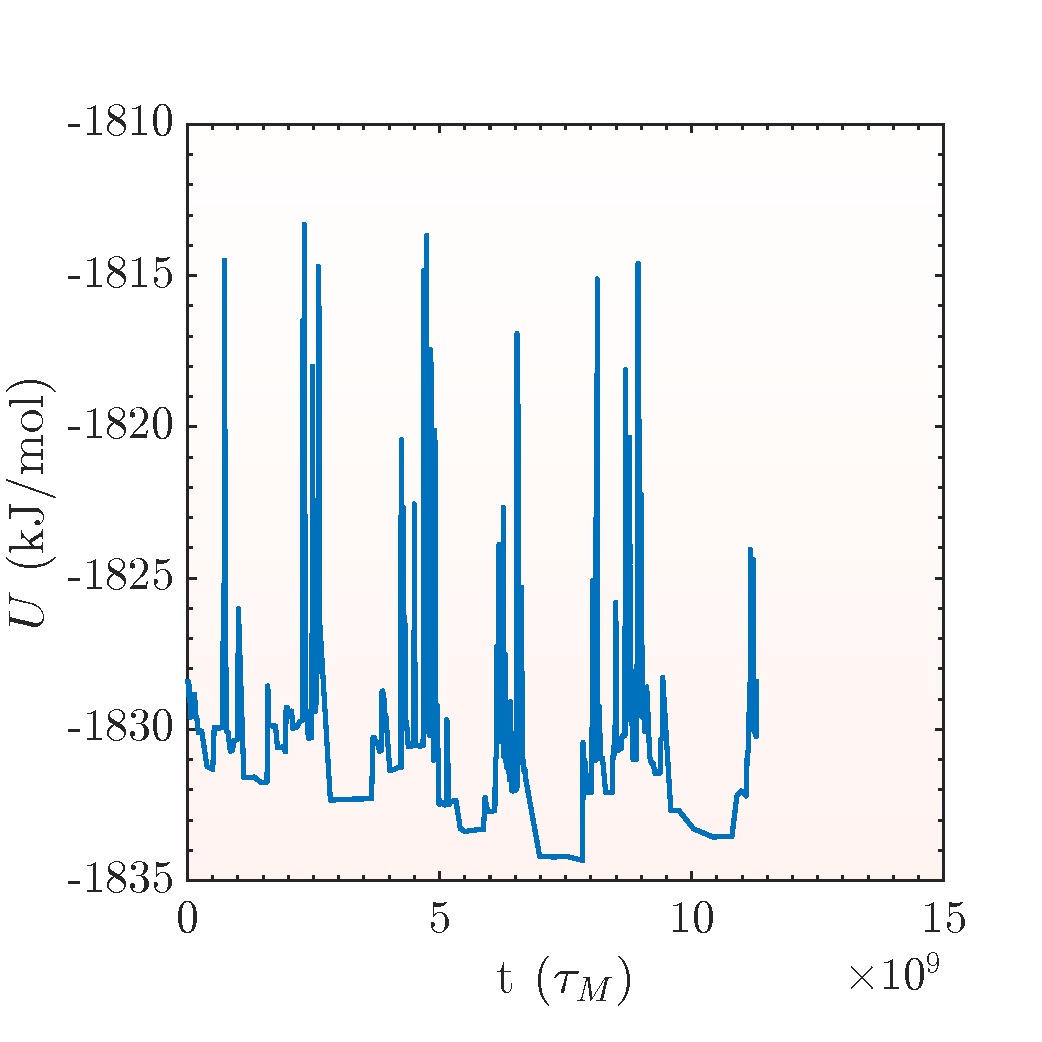
\includegraphics[width=.45\textwidth]{./Figures/Landscape/glassy_time.pdf}
	\hspace{.01\textwidth}
	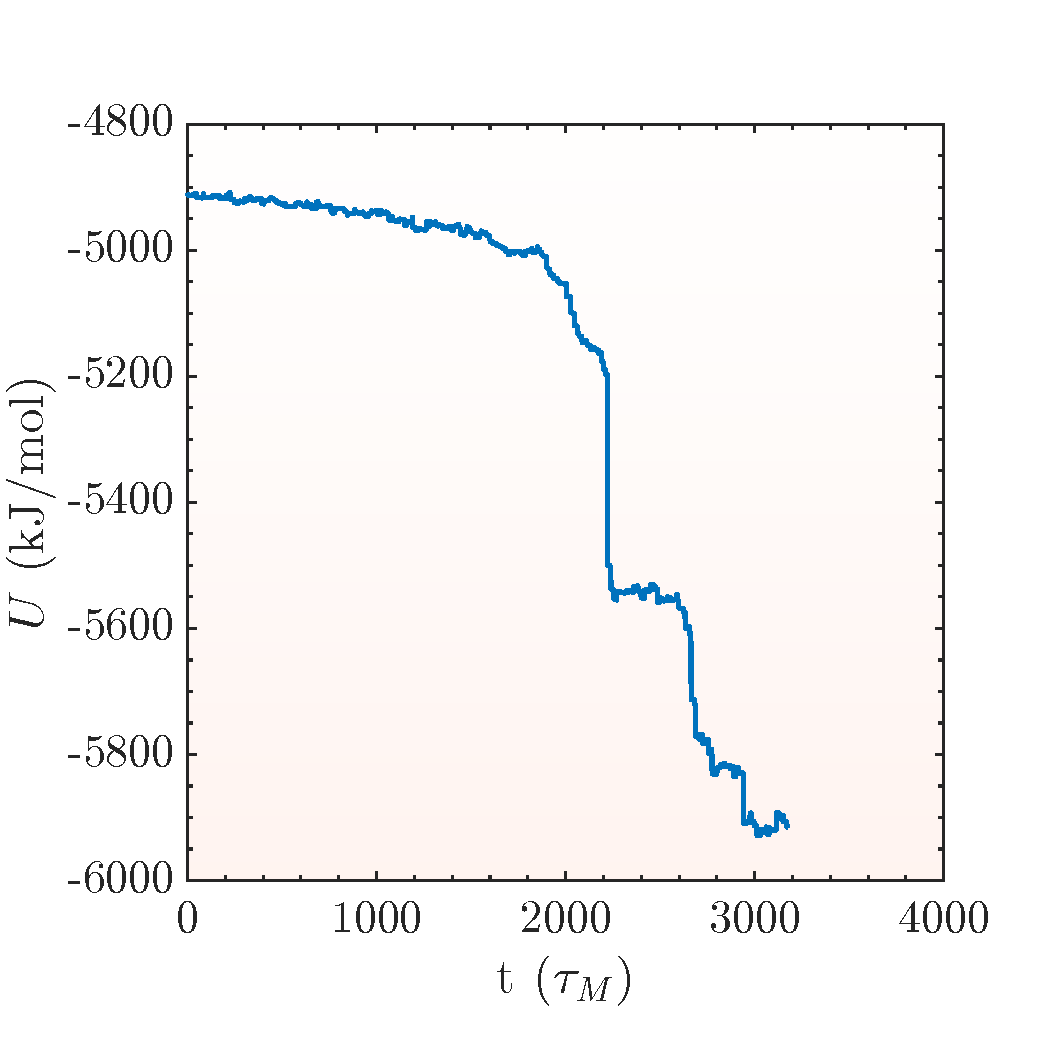
\includegraphics[width=.45\textwidth]{./Figures/Landscape/crystal_time.pdf}
	\caption{Potential Energy versus penalty number for two simulations.  The left figure shows the potential energy sampled for a binary Lennard-Jones system known for being a fragile glass former.  The right figure shows the potential energy landscape sampled for a monoatomic Lennard-Jones system known for being a poor glass former.}
	\label{compare_time}
\end{figure}

Like in the case of the nucleation study, the landscape for the binary system can be extended to the time scale rather than as a function of penalty number.  Figure \ref{compare_time} shows the energy landscape sampled as a function time.  The time scale has not been adjusted to real time units, rather it is still in terms of the Maxwellian relaxation time for the system.  As the figure shows, the binary system has a time scale orders of magnitudes larger than the monoatomic system.  Further we can see that the monoatomic system as previously shown samples gradually along the landscape in time.  Whereas, the binary system has very clear long time periods in which the system is stuck in a deep metastable state.  Similarly, the binary system when overcoming a large barrier spends very little time in the high energy state and quickly becomes stuck in a metastable basin again.  This shows that glassy dynamics are very explainable by the energy landscape.  Small time scale relaxations are related to the small energy basins within a deep metastable state, and long time relaxations are dominated by extremely large energy barriers separating deep energy basins.  

By showing the different aspects of the energy landscape for good glass formers, good crystal formers, and different densities of a good crystal former, we can use metadynamics to sample the energy landscape of a system and make predictions about the systems behavior.  The landscape can show if the system is a good glass or crystal former.  The landscape can predict rates invovled in the system, and can provide energy barriers of different timescales.